\section{Web interface}\label{sec:ui}

A basic web interface is provided to facilitate the comparison of the models explored in this thesis.
However, the focus of this work is on the methods and not on the application.
The tool consists of a backend and a frontend which are described in \autoref{subsec:backend} and \autoref{subsec:frontend}.

\subsection{Backend}\label{subsec:backend}

% this work: endpoints
The framework used for the backend is \flask{}.
%In this work, only the \texttt{GET} method is used.
There are multiple endpoints, which are used to retrieve data from the server:

\begin{itemize}
    \item \label{pt:docs}Documents: 
        Returns a list of documents, which best match the query.
        The information returned for each document is the respective \texttt{id}, \texttt{path}, and \texttt{text}.
        The query can be of type \texttt{match\_all}, which returns all documents in the database, 
        or a fuzzy full-text query if \texttt{text} is specified, 
        or a \ac{knn} query on a certain field of the database if both \texttt{knn\_type} and \texttt{knn\_source} are given.
        Moreover, the number \texttt{count} and start index \texttt{page} of the results returned can be specified.
        By default, the first 10 documents are returned.

    \item \label{pt:doc}Document: 
        Returns the metadata, i.e.\ text and path, of a document with the specified \texttt{id}.
        The \ac{url} to access this endpoint is \texttt{/documents/<id>}.

    \item \label{pt:be_pdf}PDF: 
        Returns the PDF file.
        %In order to access the path information necessary a query for a document with the specified \texttt{id} is performed.
        This endpoint is used to display the PDF in the detail component of the frontend.
        The \ac{url} to access this endpoint is \texttt{/documents/<id>/pdf}.
    
    \item \label{pt:wordcloud}WordCloud: 
        Returns the bytes of a \wordcloud{} image. 
        Depending on additional parameters, the \wordcloud{} is either generated from one document or 
        a group of similar documents.
        If the \texttt{knn\_type} is specified, a query for the \texttt{count} most similar documents is performed.
        By default, \texttt{count} is 10.
        The \ac{url} to access this endpoint is \texttt{/documents/<id>/wordcloud}.

    \item \label{pt:termfrequency}Term Frequency:
        Returns the term frequency calculated for the specified document.
        The \ac{url} to access this endpoint is \texttt{/documents/<id>/term\_frequency}.
        
    \item \label{pt:topic_wordcloud}TopicWordCloud:
        If \texttt{term} is specified this endpoint returns a \wordcloud{} of the terms that describe the topics most similar to the query term.
        The parameter \texttt{count} specifies the number of topics to be returned.
        Its default value is 3.
        The topics are generated by \ac{t2v}.
        The \ac{url} to access this endpoint is \texttt{/topics/wordcloud}.

    \item \label{pt:be_topic}Topics: 
        Returns the topics generated by \ac{t2v}. 
        The topics are described by the words closest to the topic vectors.
        The \ac{url} to access this endpoint is \texttt{/topics}.
\end{itemize}

%In order to test the endpoints during development, a swagger documentation for every endpoint is provided.





\subsection{Frontend}\label{subsec:frontend}

The framework used for the frontend is \angular{}.
There are three main components, which are used to display the data:

\begin{itemize}
    \item \label{pt:home}Home: 
        The home component is used to display the results of a text query.
        It consists of a search bar, which is used to enter the query term, and a list of results.
        If no text query is entered the first documents of the database, i.e.\ the result of a \texttt{match\_all} query, are displayed.
        The search component is shown in \autoref{fig:home_comp}.

    \item \label{pt:detail}Detail: 
        The detail component is used to display the details of a document.
        The document name and ID are located on the left side of the screen.
        Beneath the document name and ID, a button which opens the term frequency image on a new page is located. 
        Moreover, the \wordcloud{} of the document is displayed.
        The \wordcloud{} is generated from the text of the document.
        On the right side of the screen, there is a PDF viewer which displays the pages of the document.
        Beneath the PDF viewer, the file names and a \wordcloud{} of the most similar documents are displayed after a query for them is initiated by the user.
        The detail component is shown in \autoref{fig:detail_comp}.

    \item \label{pt:topic}Topic: 
        The topic component is used to display the topics of the documents.
        The topics are lists of words generated by \texttt{top2vec}.
        The user can query for the most similar topics to a term.
        The results are displayed as a \wordcloud{}.
        The upper limit of the number of topics can be defined by the user.
        The topic component is shown in \autoref{fig:top2vec_topic_comp}.
\end{itemize}


\begin{figure}[!htp] % htp = hier (h), top (t), oder auf einer eigenen Seite (p).
    \centering
    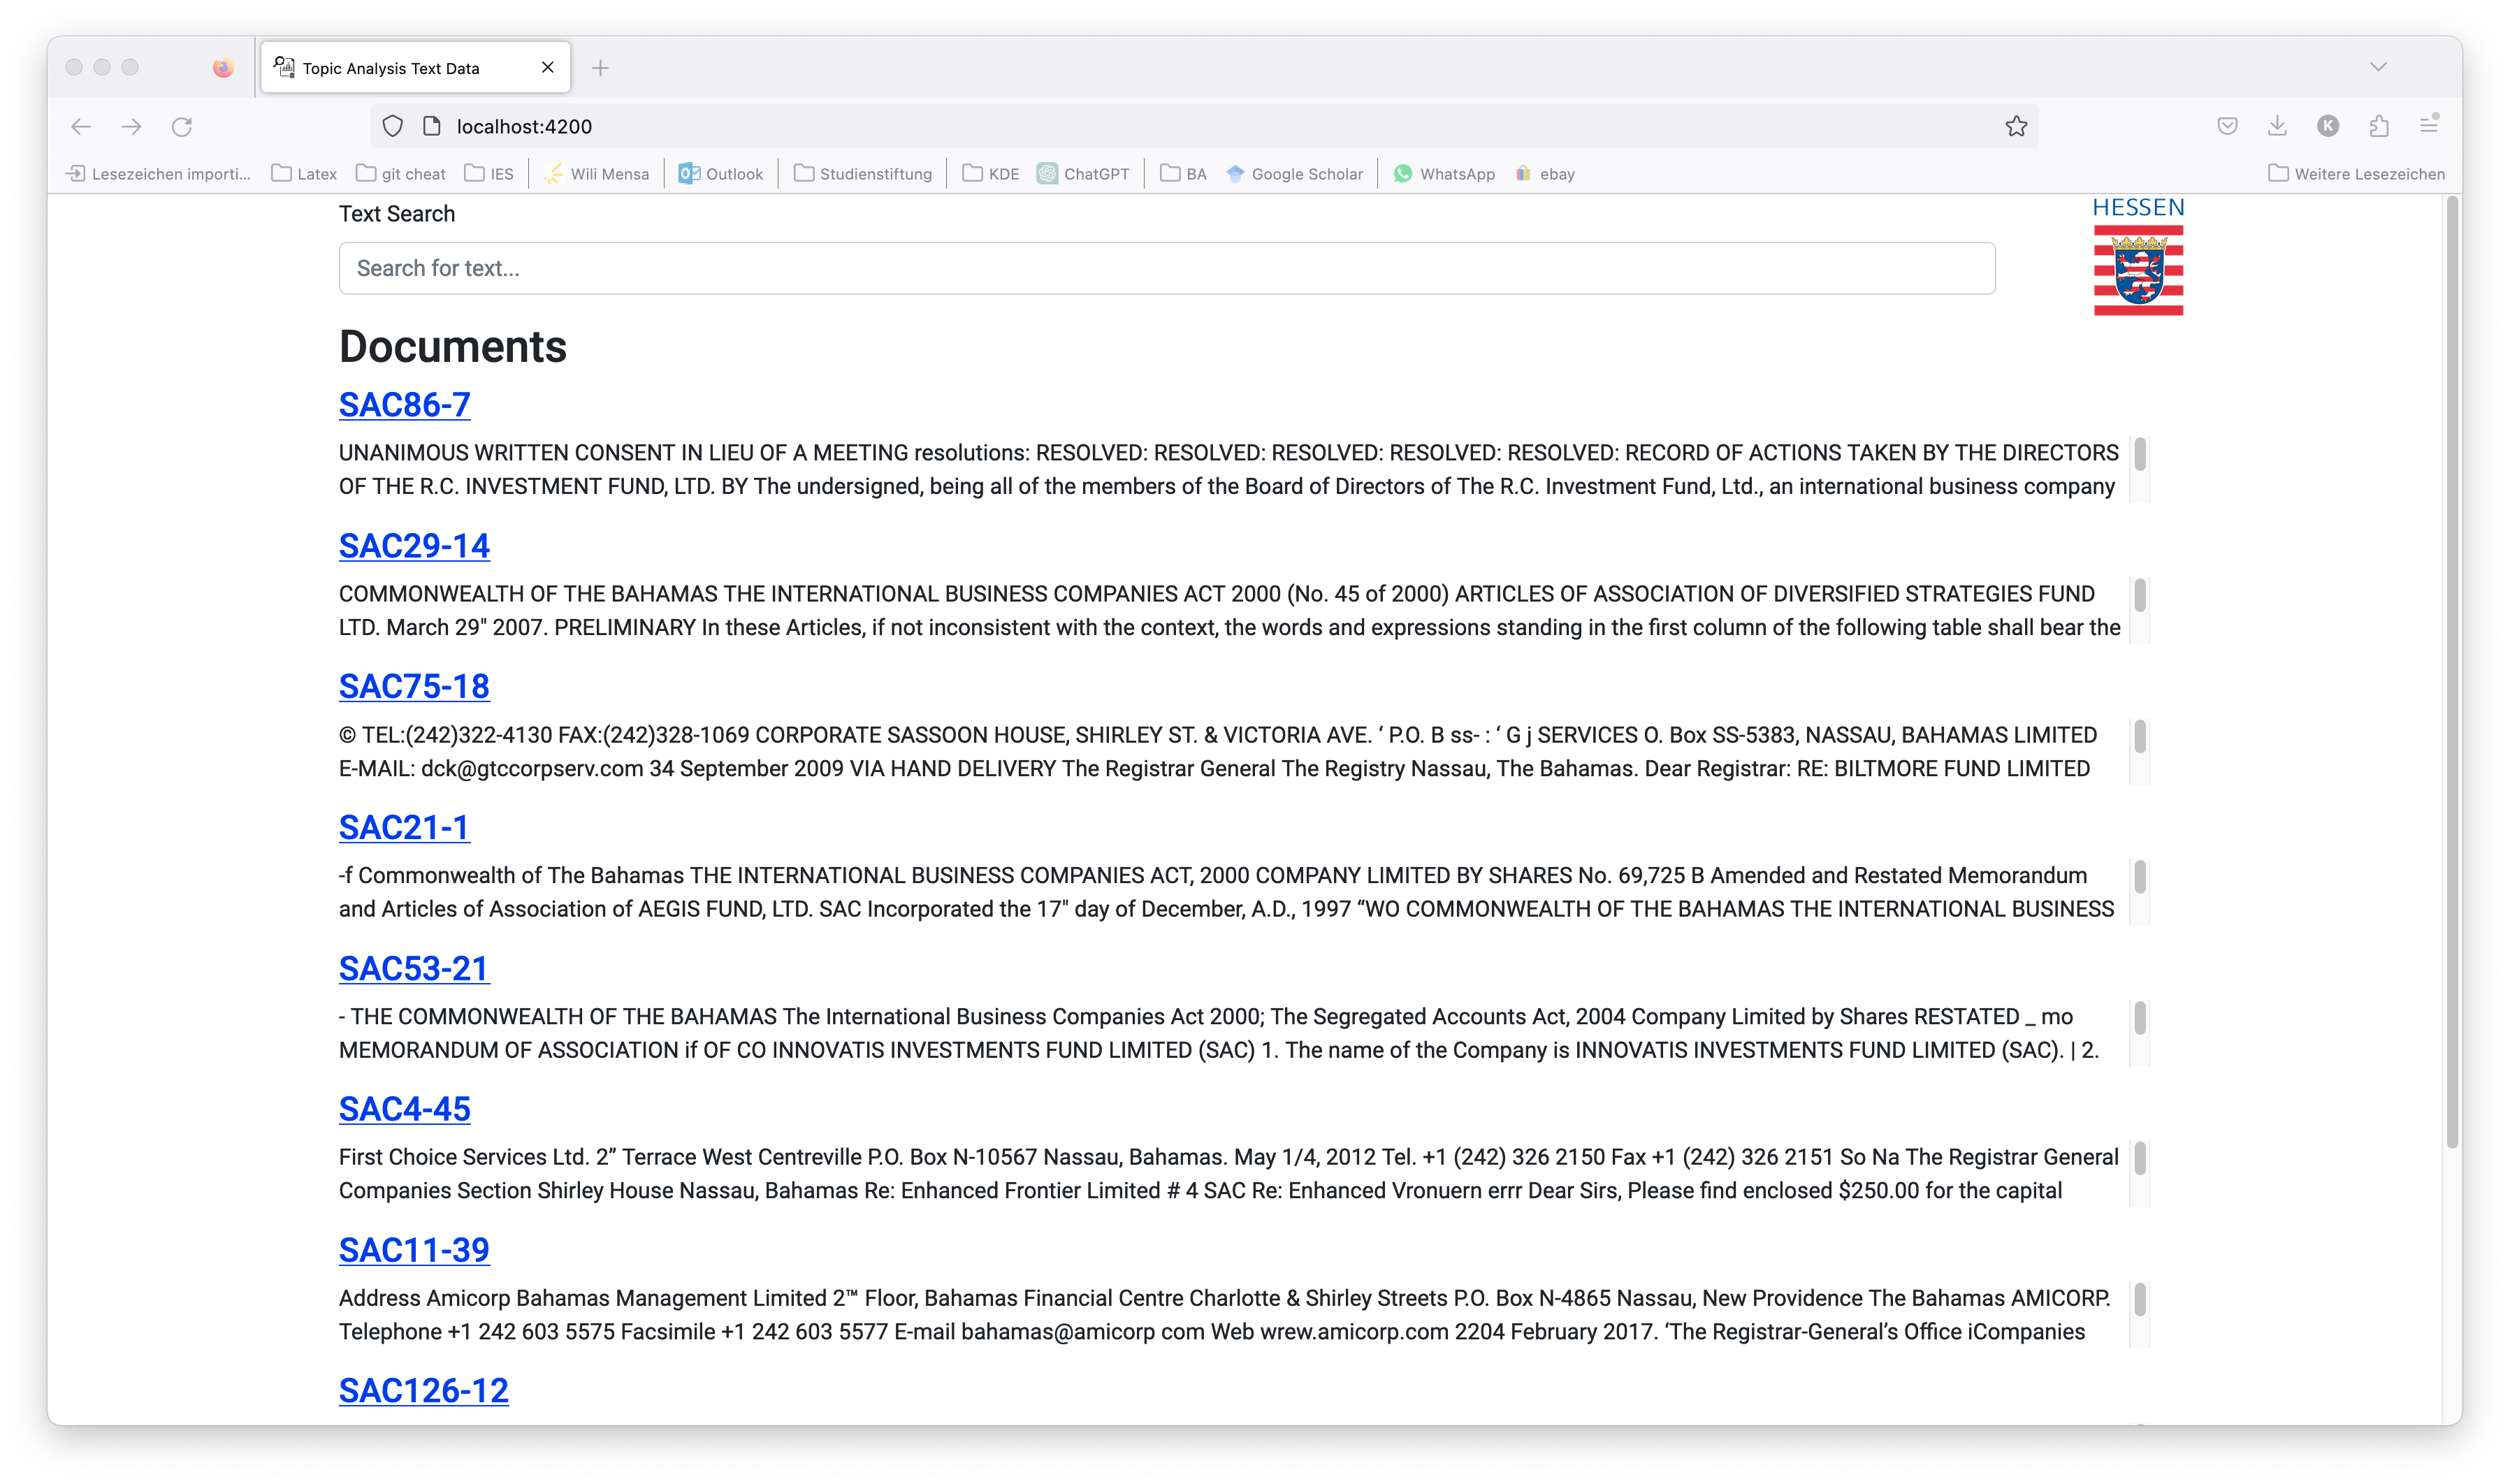
\includegraphics[width=1\textwidth]{images/UI/Home_component.png}
    \caption[Home component of the frontend]{Home component of the frontend.
    The search bar is used to enter the text query.
    The results of the query are displayed below the search bar.
    }
    \label{fig:home_comp}
\end{figure}

\begin{figure}[!htp] % htp = hier (h), top (t), oder auf einer eigenen Seite (p).
    \centering
    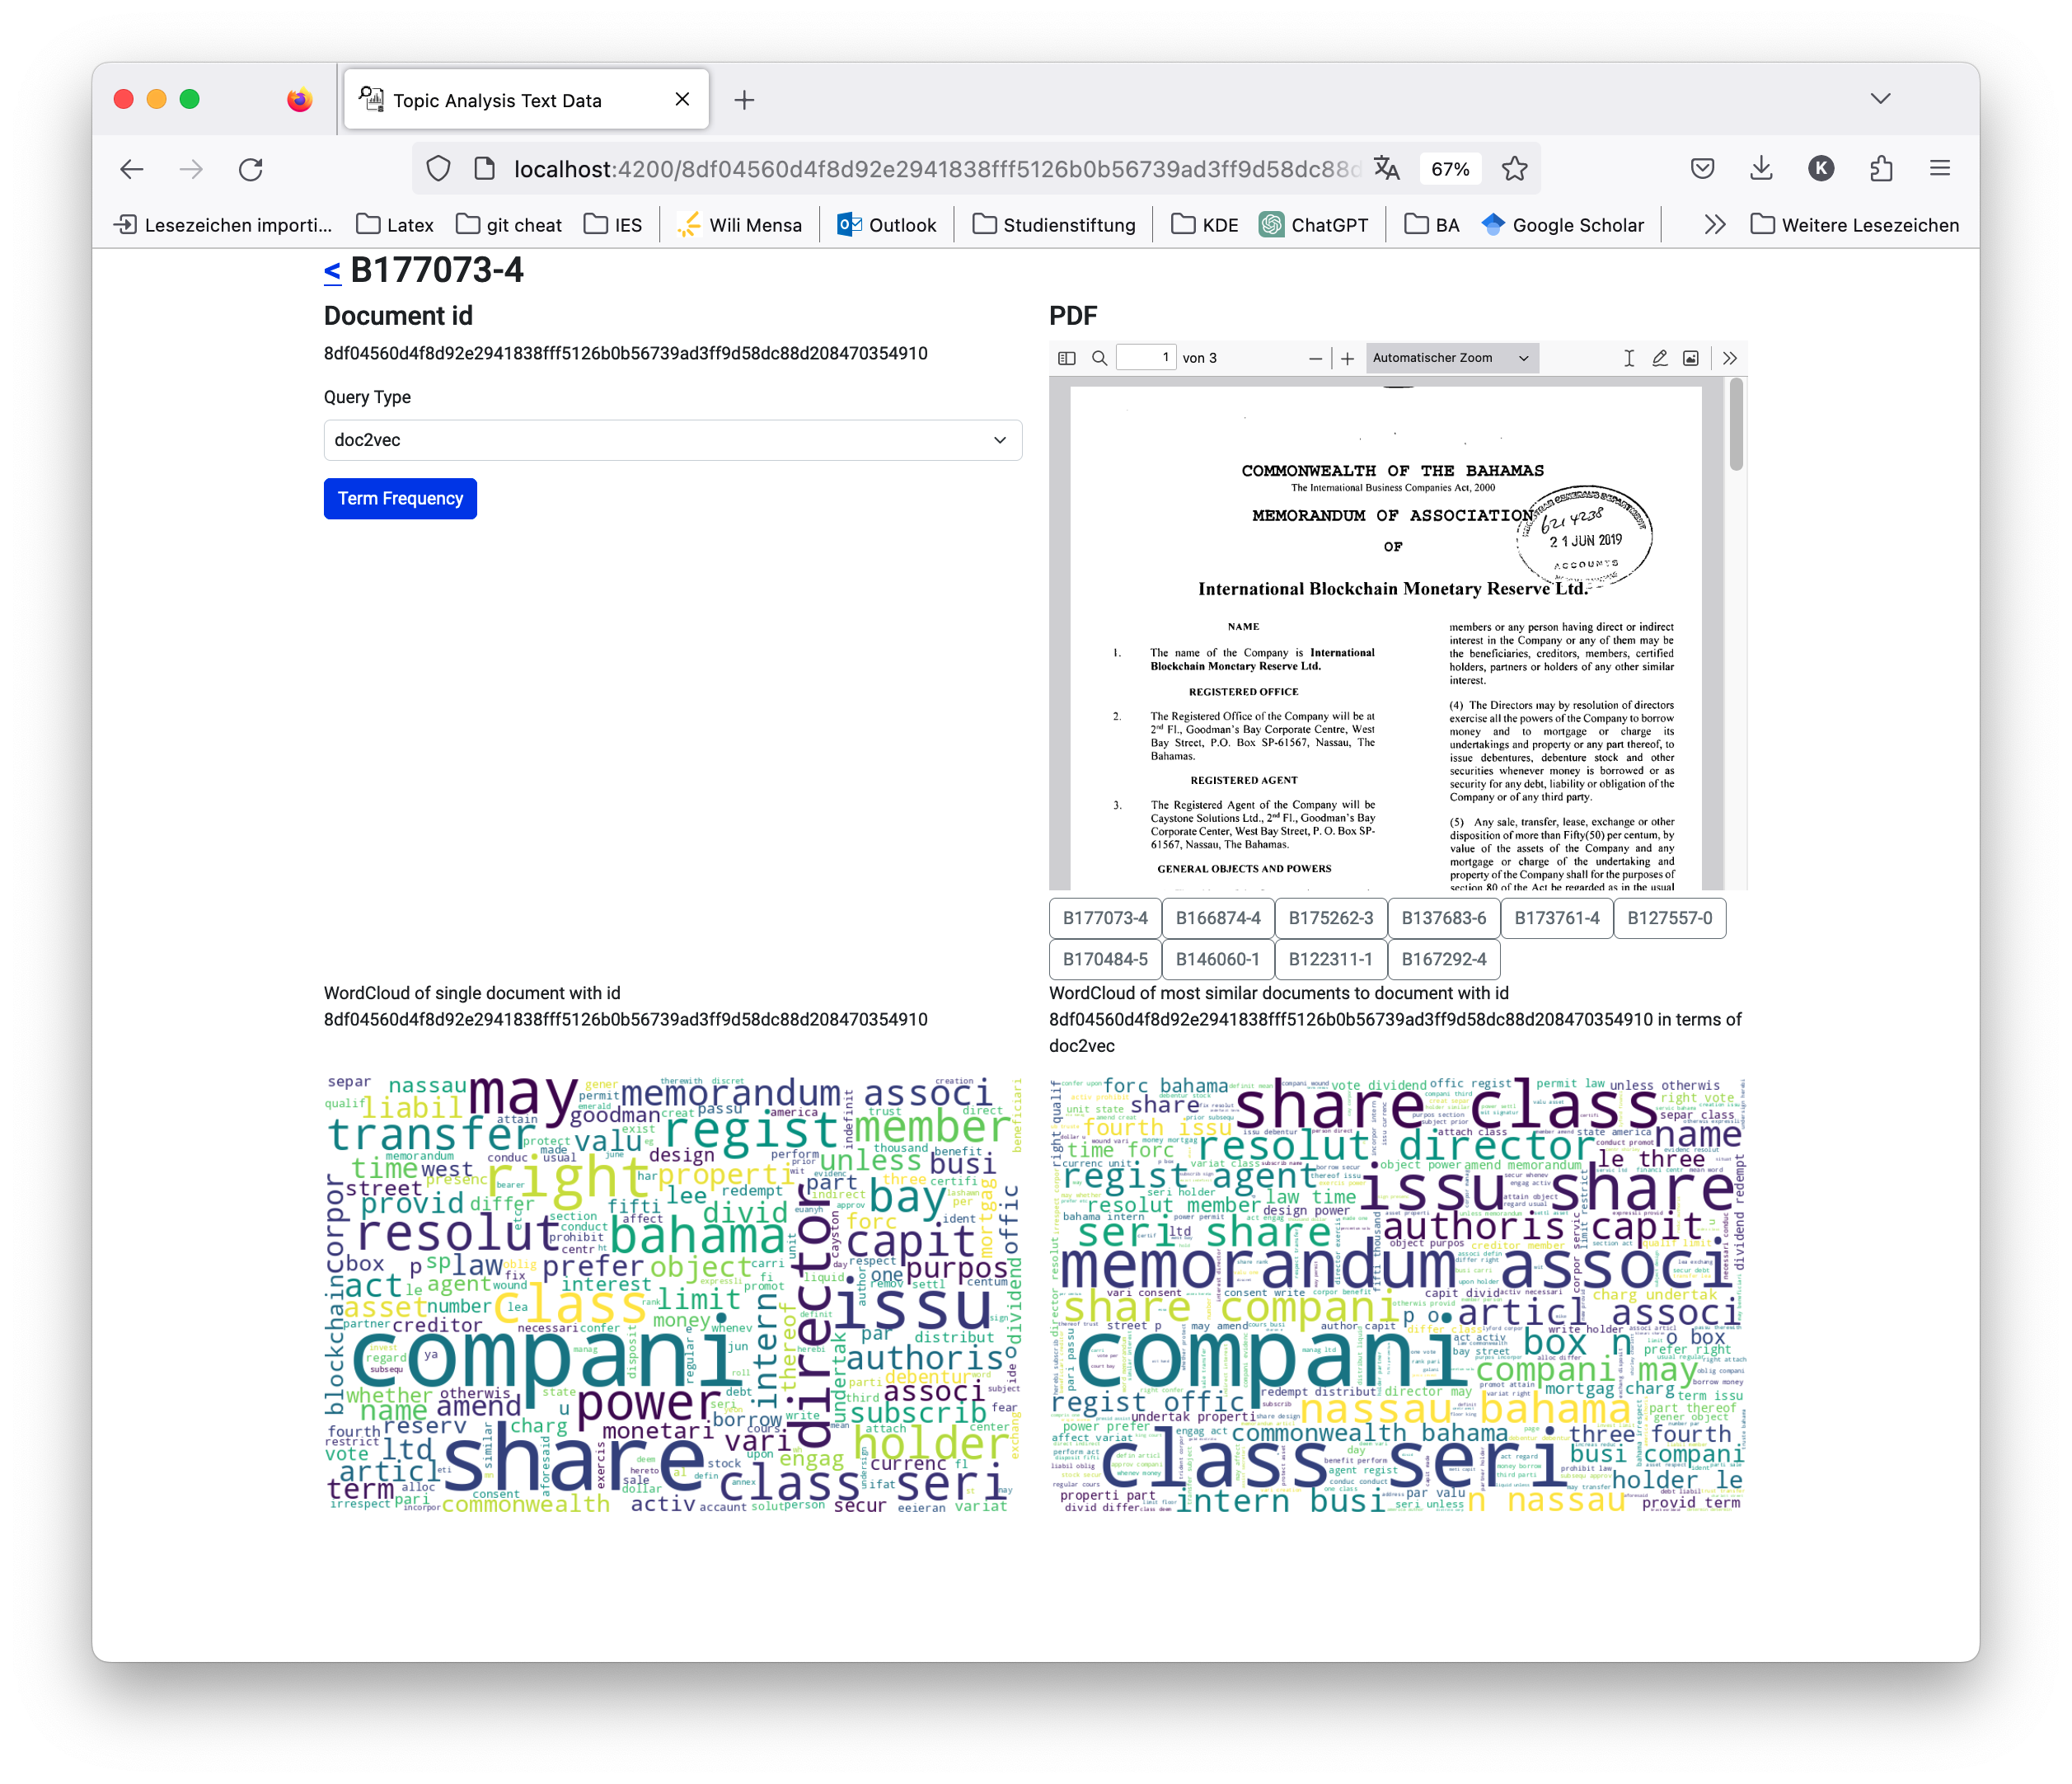
\includegraphics[width=1\textwidth]{images/UI/Home_detail.png}
    \caption[Detail component of the frontend]{Detail component of the frontend.
    The chosen document is displayed, as well as its most similar documents in the database.
    The \wordcloud{}s of the document and the most similar documents are displayed.
    }
    \label{fig:detail_comp}
\end{figure}

\begin{figure}[!htp] % htp = hier (h), top (t), oder auf einer eigenen Seite (p).
    \centering
    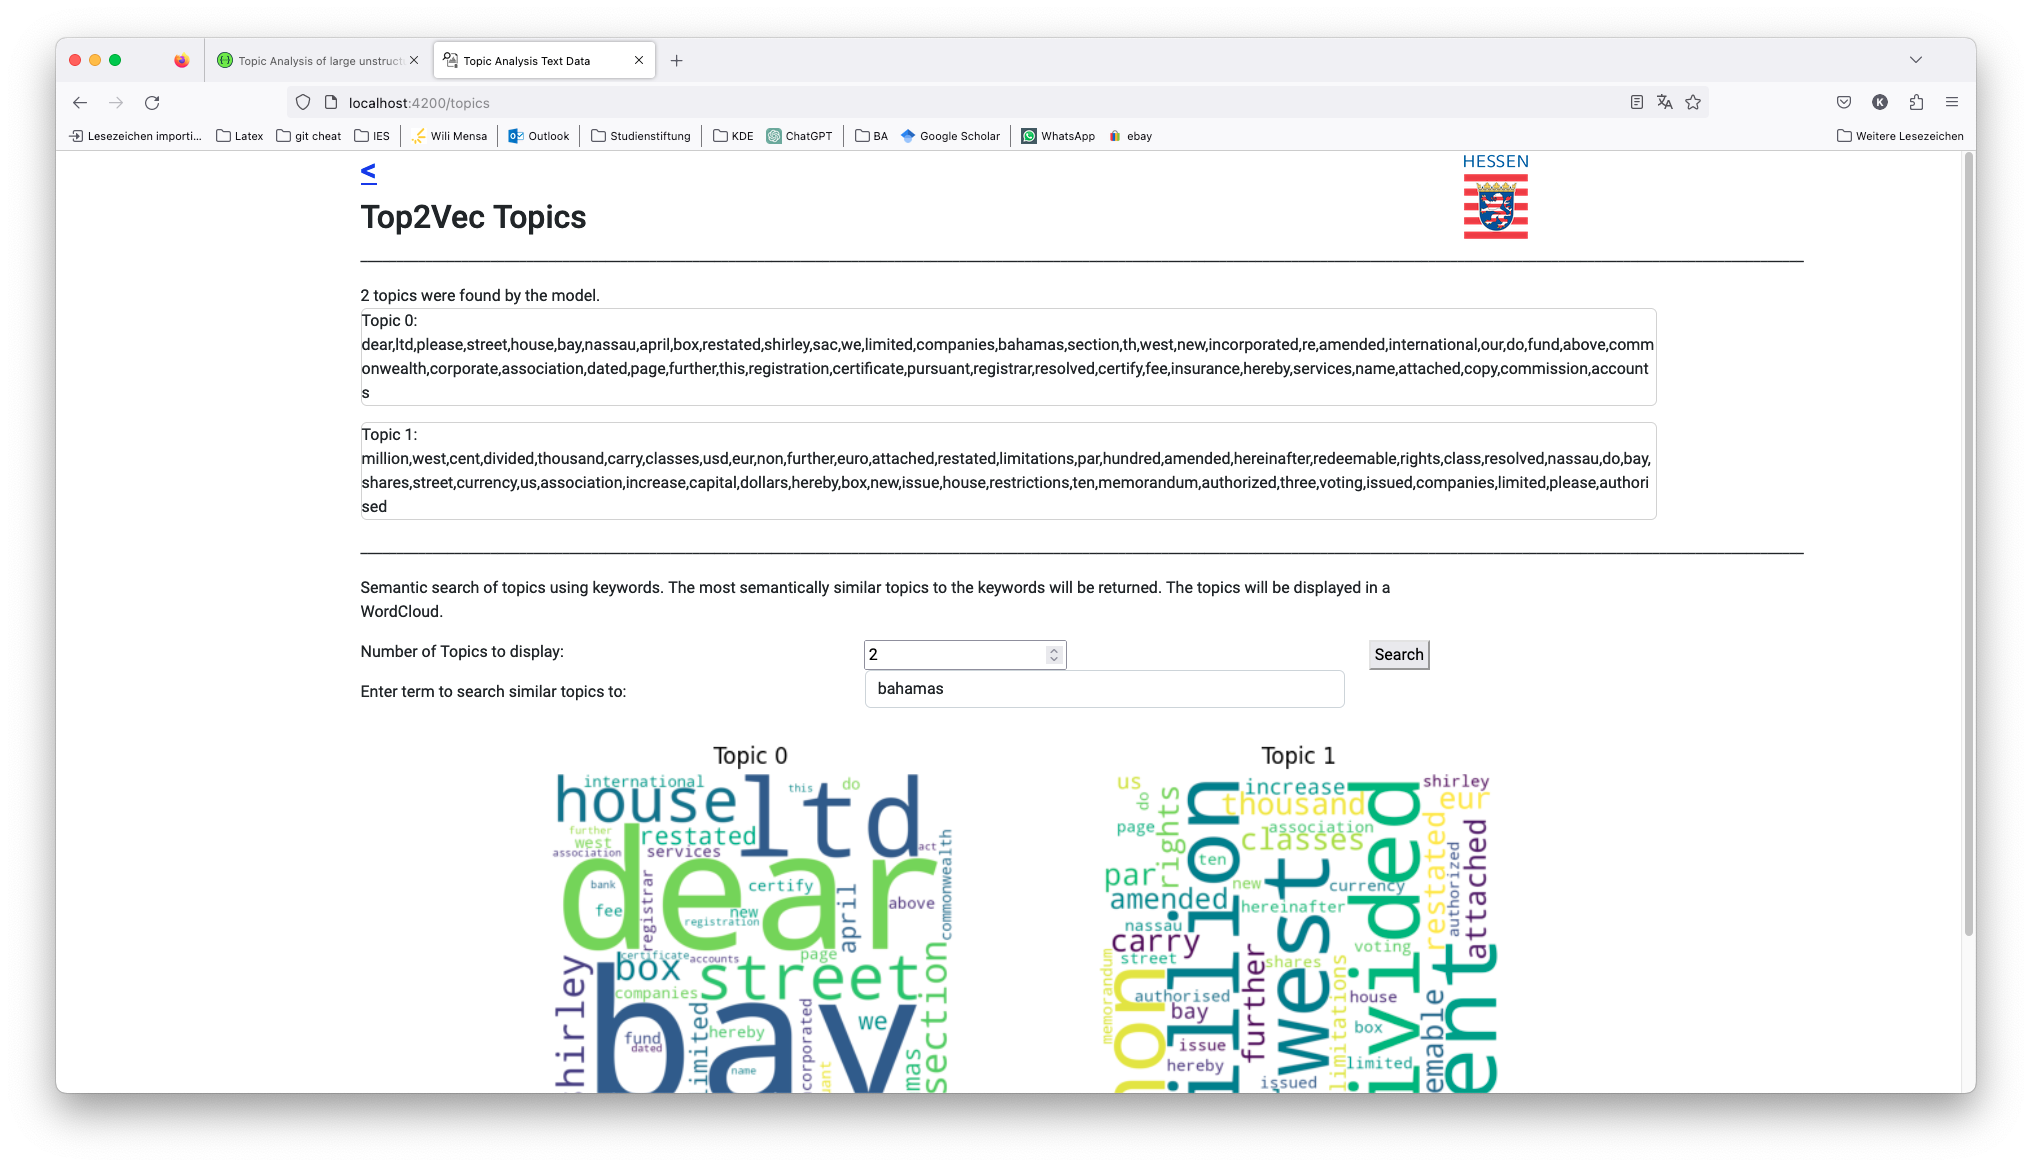
\includegraphics[width=1\textwidth]{images/UI/Top2Vec_Topics.png}
    \caption[Topic component of the frontend]{Topic component of the frontend.
    The topics identified by \acs*{t2v} are listed.
    Below them, the user can query for the most similar topics to a term.
    The results are displayed as a \wordcloud{}.
    }
    \label{fig:top2vec_topic_comp}
\end{figure}